\let\negmedspace\undefined
\let\negthickspace\undefined
\documentclass[journal]{IEEEtran}
\usepackage[a5paper, margin=10mm, onecolumn]{geometry}
\usepackage{lmodern} % Ensure lmodern is loaded for pdflatex
\usepackage{tfrupee} % Include tfrupee package

\setlength{\headheight}{1cm} % Set the height of the header box
\setlength{\headsep}{0mm}     % Set the distance between the header box and the top of the text

\usepackage{gvv-book}
\usepackage{gvv}
\usepackage{cite}
\usepackage{amsmath,amssymb,amsfonts,amsthm}
\usepackage{algorithmic}
\usepackage{graphicx}
\usepackage{textcomp}
\usepackage{xcolor}
\usepackage{txfonts}
\usepackage{listings}
\usepackage{mathtools}
\usepackage{gensymb}
\usepackage{enumitem}
\usepackage{comment}
\usepackage[breaklinks=true]{hyperref}
\usepackage{tkz-euclide} 
\usepackage{listings}
\usepackage{gvv}                                        
\def\inputGnumericTable{}                                 
\usepackage[latin1]{inputenc}                                
\usepackage{color}                                            
\usepackage{array}                                            
\usepackage{longtable}                                       
\usepackage{calc}                                             
\usepackage{multirow}                                         
\usepackage{hhline}                                           
\usepackage{ifthen}                                           
\usepackage{lscape}
\begin{document}

\bibliographystyle{IEEEtran}
\vspace{3cm}

\title{9.9.5.10}
\author{EE24BTECH11010 - Balaji B}
% \maketitle
% \newpage
% \bigskip
{\let\newpage\relax\maketitle}
\textbf{Question:}\\
Find the area of the region included between the circle $x^2 + y^2 = 8x$ and inside of the parabola $y^2 = 4x$. \\
\textbf{Answer:}
\begin{table}[h!]
    \centering
    \begin{tabular}[12pt]{ |c| c| c|c|c|c|}
    \hline
    $X$ & 1 & 2 & 3 & 4 & 5 \\
    \hline
    $P(X)$ & $K$ & 2$K$ & 2$K$ & 3$K$ & $K$ \\
    \hline 
    \end{tabular} 

    \caption{Variables used}
    \label{tab1-1.2-20}
\end{table} 

The general equation of Circle is given by 
\begin{align}
    \norm{\vec{x}}^2 + 2\vec{u}^\top \vec{x} + f = 0
\end{align}
The parameters of the given circle is 
\begin{align}
    \vec{u} = \myvec{-4 \\ 0 }, f = 0
\end{align}
Substituting the parameters of the circle in general equation, we get
\begin{align}
    \norm{\vec{x}}^2 + 2\myvec{-4 & 0}\vec{x} + 0 = 0
\end{align}
To find the point of intersection of parabola and circle, substitute parabola in circle.
\begin{align}
    \because \vec{x} = \myvec{x \\ y}
\end{align}
The parabola can be represented as
\begin{align}
    y = \pm 2\sqrt{x}
\end{align}
Substituting this in above $\vec{x}$, we get 
\begin{align}
    \vec{x} = \myvec{x \\  \pm 2\sqrt{x}}
\end{align}
Substituting this in circle, we get
\begin{align}
    \norm{\myvec{x \\ \pm 2 \sqrt{x}}}^2 + 2 \myvec{-4 & 0}\myvec{x \\ \pm 2\sqrt{x}} + 0 = 0\\
    \therefore x(x-4) = 0\\
    \implies x = 0,4
\end{align}
The point of intersection of circle and parabola can be given by
\begin{align}
    \vec{x}_1 = \myvec{0 \\ 0}\\
    \vec{x}_2 = \myvec{4 \\ 4}\\
    \vec{x}_3 = \myvec{4 \\ -4}
\end{align}
Thus, the desired Area is given as
    \begin{align}
    A &= 2\sbrak{\int_{0}^{4}\sqrt{4x}dx + \int_{4}^{8}\sqrt{8x - x^2} } \\
    A &= 2\sbrak{\sbrak{\frac{4}{3} x^{\frac{3}{2}}}_{0}^{4} + \sbrak{\frac{x-4}{2}\sqrt{8x - x^2} + 8 \sin^{-1}\brak{\frac{x-4}{4}}}_4^8 }\\
     A &= \frac{64}{3}+ 8 \pi
\end{align}
$\therefore$ The Area $A$ is $\frac{64}{3} + 8\pi$
\begin{figure}[h!]
   \centering
   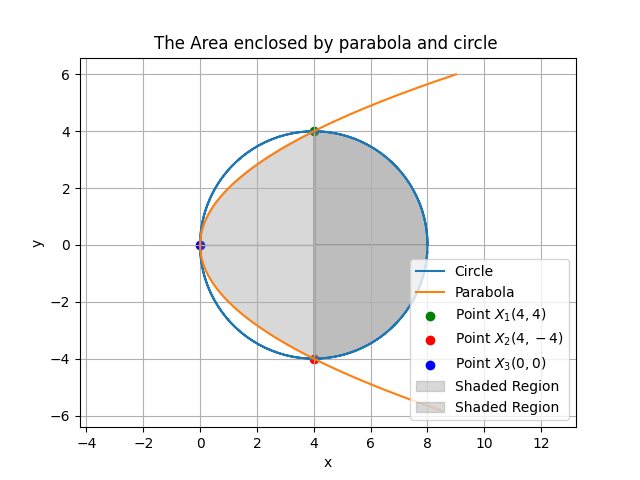
\includegraphics[width = .7\linewidth]{figs/fig.png}
   \caption{The Area enclosed by parabola and circle}
   \label{stemplot}
   \end{figure}

\end{document}
